\chapter{Soll-Zustand}\label{ch:sollzustand}
In diesem Kapitel wird auf Basis des analysierten Ist-Zustands ein Lösungskonzept für die Testdatengenerierung in automatisierten Tests für das \ac{CIF} erarbeitet und vorgestellt.

\section{Anforderungsanalyse}\label{sec:anforderungen}
Um mit dem Projekt der automatischen Testdatengenerierung einen effektiven Mehrwert für FNT bieten zu können, muss zunächst analysiert werden, welchen Anforderungen es entsprechen soll. Diese Anforderungen setzen einen Rahmen und bezeichnen einige erste Regeln und Wegweiser für die spätere Erstellung eines konkreten Lösungskonzepts, sodass dieses nachhaltig das Ziel des Projekts verwirklichen kann, eine nahezu vollständige Automatisierung der Tests durch generierte Testdaten zu erreichen. Im Folgenden sind die Anforderungen an die automatische Testdatengenerierung aufgelistet.

\begin{itemize}
    \item \textbf{Ausführungszeitpunkt.} Die Testdatengenerierung soll vor den Tests stattfinden, sodass die Testdaten bei Ausführung der Tests vollständig abrufbar sind.
    \item \textbf{Testdatenabdeckung.} Testdaten für sämtliche testdatenbezogene Tests des CIF sollen, so weit wie möglich, automatisch generiert werden.
    \item \textbf{Automatisierungsgrad.} Es sollen nach der Implementation nahezu keine händischen Schritte in Bezug zu Testdaten mehr nötig sein.
    \item \textbf{Dokumentation.} Das Projekt muss ausführlich dokumentiert sein, damit es einfach nachvollziehbar, erweiterbar und wartbar ist.
    \item \textbf{Umgebungsbereinigung.} Testdaten sollen automatisch nach der Testausführung wieder gelöscht werden. Die Testumgebung sollte nach der Ausführung so weit möglich in ihren Ausgangszustand zurückkehren.
    \item \textbf{Direkteinbindung.} Die automatische Testdatengenerierung soll direkt in das bestehende Testprojekt eingebunden werden - gemäß dem Prinzip \enquote{läuft das \ac{CIF} Automated Tests Projekt, so läuft auch die Datengenerierung}.
    \item \textbf{Unabhängigkeit.} Die Testdatengenerierung soll unabhängig von der zu testenden \textit{Command}-Instanz funktionieren.
    \item \textbf{Performance.} Es soll zu keinen erheblichen Performance-Einbußen durch die automatische Testdatengenerierung kommen. Mit leichten Einbußen durch die benötigte Zeit zur Datengenerierung ist aber zu rechnen.
    \item \textbf{Komplexität.} Es sollen nur so viele Testdaten und nur so detailreich wie nötig generiert werden, um Performance und Komplexität des Projekts zu optimieren.
\end{itemize}

\section{Analyse der benötigten Testdaten}\label{sec:testdatenanalyse}
Im nächsten Schritt erfolgt eine Analyse des \acf{SUT}. Es muss genau festgehalten werden, welche Arten von Testdaten benötigt werden und in welcher Anzahl. Ebenso muss deren Beschaffenheit und das erforderliche Verhalten zum Erzielen des gewünschten Programmablaufs berücksichtigt und dokumentiert werden. 

Hierfür wurde eine Testdatenmatrix (s. Anhang \nameref{app:testdatamatrix}) erstellt, in welcher sämtliche benötigten Testdaten erfasst werden können. Die Gesamtmatrix setzt sich aus fünf in einzelnen Seiten organisierten Teilmatrizen zusammen, welche jeweils die Testdaten für eine bestimmte Gruppe von Testobjekten beschreiben. Diese Gruppierung dient dem einfacheren Überblick und erlaubt es, Testobjekte mit ähnlichem Verhalten zusammenzufassen.

Die Teilmatrix \enquote{Device Data} ist die umfangreichste Testdatenmatrix und soll für die spätere prototypische Realisierung des Projekts die größte Rolle spielen. In ihr sind verschiedene in \textit{Command} mögliche zu testende Geräte-Entitäten, auch Hardware genannt, abgebildet, beispielsweise sogenannte \enquote{Equipments} wie \enquote{Chassis}, aber auch die Entitäten \enquote{Network Element} und \enquote{Switch Cabinet}. Diese Entitäten können in \textit{Command} in eine Zone, also einen Campus, ein Gebäude, ein Stockwerk oder einen Raum platziert werden und über das \ac{CIF} entsprechend verschiedener Deltafälle aktualisiert oder gar gelöscht werden. Ebenfalls können Devices in eine \ac{NMS}-Tabelle geladen werden, um die Datenintegration von einem Fremdsystem darzustellen. Das Ziel der Testdaten ist es zunächst, die Devices in einem für \textit{Command} validen Format abzubilden, sodass diese überhaupt platziert werden können, beziehungsweise auch valide für die \ac{NMS}-Tabelle des Hardwaretyps, um die Daten in diese laden zu können. Dieser Vorgang wird in Kapitel \ref{sec:loesungskonzept} näher erläutert. Darauf aufbauend sollen die Testdaten genau die in der Matrix definierten Deltafälle auslösen, sodass die Deltaberechnung des \ac{CIF} verlässlich getestet werden kann. Um dies zu erreichen, müssen die Daten veschiedene Anforderungen erfüllen. Diese Anforderungen werden in der Testdatenmatrix durch die Spalten \enquote{NMS} und \enquote{Command} beschrieben und richten sich nach den offiziellen für \textit{Command} definierten Deltafall-Use-Cases. \cite{fntusecases:2022}

Ein \enquote{X} in der Spalte \enquote{NMS} bedeutet, dass für das Auslösen des betrachteten Deltafalls ein Objekt in der zugehörigen \ac{NMS}-Tabelle vorhanden sein muss. Etwas Ähnliches gilt für die Spalte \enquote{Command}; hier bezeichnet das \enquote{X} ein in \textit{Command} platziertes Objekt.

Nur mit Vorhandensein eines Objekts in den benötigten Tabellen sind die Anforderungen an die meisten Deltafälle allerdings nicht erfüllt. Zunächst ist zu beachten, dass für jeden Deltafall, bei dem mehrere Objekte in verschiedenen Tabellen gleichzeitig vonnöten sind, die Objekte ein Attribut aufweisen müssen, mit dem sie bei der Deltaberechnung erkannt und gruppiert werden können. Dieses Attribut wird bei den Geräten durch die sogenannte \textit{visibleId} dargestellt. Diese muss für die Erkennung eines bestimmten Deltafalls für alle zugehörigen Objekte, obgleich sie in verschiedenen Tabellen gespeichert sind, identisch sein.

Weiterhin müssen die Testobjekte für manche Deltafälle unterschiedliche Attributwerte aufweisen und für andere Deltafälle wiederum identisch sein. Hierfür kann das Symbol \enquote{X} auch Erweiterungen tragen; die kleinen Buchstaben \enquote{a}, \enquote{b} oder \enquote{c} hinter dem \enquote{X} bezeichnen hierbei, dass es sich bei den Objekten \enquote{Xa}, \enquote{Xb} und \enquote{Xc} um Objekte mit gleicher \textit{visibleId}, aber unterschiedlichen Attributen handelt.

Schließlich müssen sich zum Testen der Plan-Deltafälle manche Objekte in \textit{Command} im Planungsstatus, entweder \enquote{PLANNED\_DELETED} oder \enquote{PLANNED\_CREATED}, befinden. Dies wird durch eine weitere Ergänzung des \enquote{X}-Symbols dargestellt. Ein \enquote{-} bezeichnet ein Objekt mit Planstatus \enquote{PLANNED\_DELETED}, während ein \enquote{+} den Status \enquote{PLANNED\_CREATED} abbildet.

\section{Analyse der benötigten Tools}\label{sec:toolanalyse}
Eine umfassende Analyse der bestehenden Tool-Landschaft vor dem ersten Entwurf eines Konzepts ist immer sinnvoll. Wird ein bereits existierendes Software-Tool gefunden, welches genau die benötigten Anforderungen abdeckt, können eine Vielzahl von Ressourcen, wie Zeit und Kapital, die zum Entwickeln eines In-House-Tools nötig wäre, eingespart werden. 

\subsection{Detailgrad der Analyse}\label{toolanalysedetail}
Für eine effektive Toolanalyse muss der Umfang des Projekts erfasst werden. Es ist wichtig, bei der Toolanalyse zu wissen, mit wie vielen Benutzern das geplante Programm in Berührung kommen soll, um den Detailgrad der Analyse abzustimmen. Eine überaus formelle und detaillierte Toolanalyse für ein Programm, welches nur von einzelnen Personen verwendet wird, würde unnötig viel Aufwand bereiten, während genau dies für ein sehr großes Projekt definitiv notwendig ist. Ein potentielles Tool muss dabei exakt zu den aufgestellten Anforderungen passen. \cite[S. 249]{fewster:1999} Im Fall der automatischen Datengenerierung für die automatisierten Tests des \ac{CIF} gilt, dass die Tests zwar nur von einigen wenigen Entwicklern ausgeführt werden. Jedoch bilden sie die Basis zur Validierung der korrekten Funktion des \ac{CIF}, welches wiederum von vielen Kunden und deren Mitarbeitern verwendet wird. Das Projekt betrifft so indirekt eine große Anzahl von Nutzern; es sollte also eine ausführliche und detaillierte Toolanalyse durchgeführt werden.

\subsection{Formulieren der Anforderungen an ein Tool}\label{toolanalyseanforderungen}
Bevor überhaupt nach einem Tool gesucht werden kann, müssen Anforderungen an dieses formuliert werden, denn diese bilden Vergleichspunkte und sind entscheidend dafür, ob ein Tool in das geplante Projekt integriert werden soll oder nicht. Wird ein Tool ausgewählt, ohne dieses zuvor auf diverse Anforderungen für die Funktionalität des Projekts zu prüfen, kann es sein, dass ein unpassendes Tool ausgewählt wird, welches in der Umgebung des Projekts nicht wie geplant oder überhaupt nicht funktioniert und so die Umsetzung des Projekts erschwert. \cite[S. 249]{fewster:1999} Gerade falls solche Komplikationen erst während der Umsetzung auftreten, sind diese dann nur sehr aufwändig und mit vielen Änderungen am Projekt zu beheben und damit ein großer Kostenfaktor.

Taheri und Sadjadi formulieren einige grundsätzliche Kriterien, die bei der Auswahl eines Softwaretools berücksichtigt werden sollten. Zwar sind diese im Kontext der Analyse von Tools zur agilen Entwicklung formuliert, jedoch können diese auch allgemein verstanden und somit ebenso auf den Themenbereich der automatischen Testdatengenerierung angewandt werden.

\begin{itemize}
    \item \textbf{Flexibilität}: Ein Tool sollte flexibel sein und sich den wandelbaren Anforderungen des Unternehmens anpassen können.
    \item \textbf{Benutzerfreundlichkeit}: Das Tool sollte einfach integrierbar und ohne lange Einarbeitungszeit benutzbar sein.
    \item \textbf{Kosten}: Der Kostenfaktor spielt eine wichtige Rolle in der Auswahl eines passenden Tools.
    \item \textbf{Responsivität}: Responsivität bezeichnet die Verfügbarkeit von Support und die Reaktivität des Herstellers eines Tools. Ist dies gegeben und wie wird auf Anfragen von Kunden reagiert?
    \item \textbf{Features}: Ein passendes Tool sollte Features beinhalten, die für das geplante Projekt einsetzbar sind.
\end{itemize}
\cite{taheri:2015}

Im speziellen Kontext der automatischen Datengenerierung ergeben sich für ein potentielles Tool also folgende Anforderungen beziehungsweise Kriterien:

\begin{enumerate}
    \item Die Datengenerierung muss einfach anpassbar sein, falls sich Funktionalitäten in \textit{Command} ändern. Dies können beispielsweise neue Entitäten oder neue Attribute sein.
    \item Das Tool soll ohne größeren Aufwand direkt in die Umgebung der \ac{CIF} Automated Tests eingebunden werden können und keine extra-Applikation nötig sein.
    \item Mit dem Tool sollen portable Tests realisiert werden können; die Testdatengenerierung soll also unabhängig von der darunterliegenden \textit{Command}-Instanz funktionieren.
    \item Das Tool soll, wenn möglich, keine Softwarekosten verursachen. Es soll also keine proprietäre Software mit hohen Lizenzkosten ausgewählt werden, da es in diesem Rahmen eher prototypisch für ein einzelnes Projekt eingesetzt wird.
    \item Ein verlässlicher Support soll verfügbar sein, da die Effektivität der Tests von der Korrektheit der automatischen Datengenerierung abhängt und Fehler hier schnell behoben werden müssen.
    \item Das Tool soll in eine \textit{Jenkins}-Build-Pipeline einbindbar beziehungsweise kompatibel mit Gradle sein.
    \item Die Testdaten sollen reale Daten in Command imitieren und müssen hierbei korrekt formatiert werden können.
    \item Die generierten Daten müssen die Vorgaben zur Deltaberechnung erfüllen können, die in Kapitel \ref{sec:testdatenanalyse} in der Testdatenmatrix formuliert wurden.
    \item Die Daten sollen nicht direkt in die Datenbank gespeichert werden, sondern über die Middleware verwaltbar und somit kompatibel mit Java und \ac{REST}-Interfaces sein, da auch die Funktionalität des Erstellens von Objekten in \textit{Command} getestet werden soll. Objekte sollen also nur über \ac{REST}-Anfragen der \ac{BGE} erstellt werden.
\end{enumerate}

\subsection{Auswahl potentieller Tools zur Datengenerierung}\label{toolanalysauswahl}
Nach ausführlicher Recherche wurden aus einer Vielzahl von verfügbaren Tools zur Datengenerierung die folgenden vier Generatoren ausgewählt. Diese Tools sind im Folgenden aufgelistet.

\begin{itemize}
    \item \textbf{Rapiddweller Benerator:} Ein umfangreiches Tool zur vollständigen Generierung oder Obfuskation von diversen möglichst realen Testdaten über zuvor defininierte Konfigurationen. \cite{benerator:2022}
    \item \textbf{Mockaroo:} Ein Online-Tool mit \ac{API}-Anbindung, über das sich reale Testdaten nach Konfiguration und sogar ganze \ac{API}s nachbilden lassen. \cite{mockaroo:2022}
    \item \textbf{Data Factory:} Eine Java-Bibliothek zum Generieren von Werten für Testdaten. \cite{datafactory:2022}
    \item \textbf{Java Faker:} Ähnlich wie \textit{Data Factory} eine Java-Bibliothek, die vielerlei Datentypen und realistische Werte für Testdaten generieren kann. \cite{javafaker:2022}
\end{itemize}

\subsection{Evaluierung}\label{toolanalysevaluierung}
Die vier präsentierten Tools sollen nun im Vergleich mit einer potentiellen In-House-Implementierung in Hinblick auf die in Abschnitt \ref{toolanalyseanforderungen} formulierten Anforderungen evaluiert werden. Die Tabelle \ref{tab:toolanalyse} zeigt die Ergebnisse dieser Evaluation grafisch aufbereitet. Eine grün gefärbte Zelle bedeutet hier, dass das Tool die Anforderung gut erfüllt, eine gelbe Färbung stellt eine mittelmäßige Erfüllung der Anforderung dar und eine rot gefärbte Zelle drückt aus, dass das Tool die Anforderung nicht oder nur schlecht erfüllt.

\begin{sidewaystable}[h!p]
    \begin{center}
        \begin{tabular}{| >{\raggedright\arraybackslash}m{16em} | >{\raggedright\arraybackslash}m{6em} | >{\raggedright\arraybackslash}m{6em} | >{\raggedright\arraybackslash}m{6em} | >{\raggedright\arraybackslash}m{6em} | >{\raggedright\arraybackslash}m{6em} |}
            \hline
              & Benerator & Mockaroo & Data Factory & Java Faker & In-House \\ 
             \hline\hline
             Einfach anpassbar & \cellcolor{good} & \cellcolor{good} & \cellcolor{good} & \cellcolor{good} & \cellcolor{good} \\ 
             \hline
             Einfache Integrierung & \cellcolor{neutral} & \cellcolor{good} & \cellcolor{good} & \cellcolor{good} & \cellcolor{good} \\ 
             \hline
             Portabilität der Tests & \cellcolor{neutral} & \cellcolor{neutral} & \cellcolor{bad} & \cellcolor{bad} & \cellcolor{good} \\ 
             \hline
             Kosten & \cellcolor{good} & \cellcolor{neutral} & \cellcolor{good} & \cellcolor{good} & \cellcolor{neutral} \\ 
             \hline
             Support & \cellcolor{neutral} & \cellcolor{neutral} & \cellcolor{bad} & \cellcolor{neutral} & \cellcolor{neutral} \\ 
             \hline
             \ac{CI}-Unterstützung & \cellcolor{good} & \cellcolor{good} & \cellcolor{good} & \cellcolor{good} & \cellcolor{good} \\ 
             \hline
             Reale Datenabbildung & \cellcolor{good} & \cellcolor{good} & \cellcolor{neutral} & \cellcolor{neutral} & \cellcolor{good} \\ 
             \hline
             Erfüllung der Dekta-Anforderungen & \cellcolor{bad} & \cellcolor{bad} & \cellcolor{bad} & \cellcolor{bad} & \cellcolor{good} \\ 
             \hline
             Testdaten in der Middleware & \cellcolor{good} & \cellcolor{good} & \cellcolor{good} & \cellcolor{good} & \cellcolor{good} \\ 
             \hline
        \end{tabular}
        \caption{Toolanalyse in Tabellenform}\label{tab:toolanalyse}
    \end{center}
\end{sidewaystable}

\subsubsection*{Einfache Anpassbarkeit}
Bei der Anpassbarkeit schneiden alle möglichen Lösungen sehr gut ab. Für Tools wie \textit{Benerator} oder \textit{Mockaroo} können die Datenkonfigurationen einfach angepasst werden und Bibliotheken wie \textit{Data Factory} und \textit{Java Faker} sind sehr leichtgewichtig und können durch die flexible Verwendung ihrer verschiedenen Generierungsmethoden einfach angepasst werden. Auch eine In-House-Lösung kann sehr flexibel implementiert werden und vor allem dadurch, dass der Programmierer den vollen Überblick über den Code hat, einfach erweitert oder anderweitig angepasst werden.

\subsubsection*{Einfache Integrierbarkeit}
\textit{Mockaroo} kann über seine \ac{API} bequem von der Middleware aus angesprochen werden, während \textit{Data Factory}, \textit{Java Faker} und eine In-House-Lösung sowieso direkt im Testprojekt eingebunden werden. Einzig \textit{Benerator} fällt in dieser Hinsicht zurück, da das Tool separat heruntergeladen, installiert und konfiguriert werden muss. Dies bedeutet, dass einige zusätzliche Schritte zur Integrierung des Tools direkt in das Testprojekt nötig sind, die bei den anderen Tools wegfallen.

\subsubsection*{Portabilität der Tests}
Beim Aspekt der Portabilität hat eine In-House-Lösung einen klaren Vorteil, denn sie kann bewusst so implementiert werden, dass sie mit verschiedenen \textit{Command}-Instanzen umgehen kann. Bei allen anderen Tools müssten zunächst selbst Abprüfungen und Abfragen beispielsweise von verfügbaren Gerätetypen implementiert werden, um den Tools eine für die zu testende Instanz valide Datengrundlage zu geben. Besonders die zwei Bibliotheken schneiden hier schlecht ab, da deren vordefinierte Methoden zur Wertegenerierung gar keine Möglichkeit haben, Daten aus einem validen Wertepool zu schöpfen, ohne selbst die Bibliotheken mit passenden Methoden zu erweitern.

\subsubsection*{Kosten}
Mit der \textit{Benerator Community Edition} existiert eine \ac{OSS}-Variante des Tools, womit Lizenzkosten entfallen. \cite{beneratorce:2022} \cite{singh:2015} \textit{Mockaroo} bietet zwar auch eine kostenlose Variante an, jedoch ist diese auf 200 \ac{API}-Anfragen pro Tag begrenzt, was bei einer größeren Testdatenmenge schnell zu knapp wird. Die günstigste Premium-Lizenz des Tools beläuft sich auf \$60 pro Jahr. Die Java-Bibliotheken \textit{Data Factory} und \textit{Java Faker} sind beide \ac{OSS} und damit kostenlos. Eine In-House-Lösung ist zwar grundsätzlich auch kostenlos, erfordert aber mehr Implementierungsaufwand als bei Verwendung eines Tools, sodass hier die länger für die Implementierung verbrachte Zeit als Kostenfaktor gerechnet werden muss.

\subsubsection*{Support}
In der Kategorie Support kann keine Lösung vollständig überzeugen. Das Problem bei \ac{OSS}-Lösungen ist, dass die Qualität des Supports von der hinter dem Tool stehenden Community abhängt. Hierbei kann nicht zuverlässig gesagt werden, wie schnell und effektiv bei akuten Problemen mit dem Tool geholfen werden kann. Besonders kritisch ist dies bei \textit{Data Factory}, da es sich um eine sehr kleine, von wenigen Personen entwickelte Bibliothek handelt. Die Chance, schnell Hilfe zu bekommen, ist dort also deutlich geringer als bei größeren Projekten. Bei einer In-House-Lösung kann prinzipiell der*die Entwickler*in sehr schnell selbst eingreifen und Probleme beheben. Jedoch besteht hier auch die Gefahr, dass ein Problem nicht schnell genug behoben werden kann, wenn der*die Entwickler*in nicht verfügbar ist.

\subsubsection*{\ac{CI}-Unterstützung}
Alle Lösungen lassen sich ohne Probleme in eine Build-Pipeline integrieren und unterstützen somit \ac{CI}.

\subsubsection*{Reale Datenabbildung}
In Bezug auf eine möglichst reale Abbildung der Testdaten haben \textit{Benerator}, \textit{Mockaroo} und eine In-House-Lösung den Vorteil, dass diese Daten auf Grundlage realer in \textit{Command} existierender Werte generieren können - sofern diese konfiguriert werden. Java-Bibliotheken wie \textit{Data Factory} und \textit{Java Faker} bringen eine solche Funktionalität nicht mit und können daher Testdaten nur zum Teil real abbilden.

\subsubsection*{Erfüllung der Delta-Anforderungen}
Die definierten Deltafälle können nicht durch die Drittanbietertools abgedeckt werden, ohne, wie schon beim Faktor Portabilität angesprochen, programmiertechnische Erweiterungen zusätzlich zur Einbindung des Tools zu erfordern. Eine In-House-Lösung kann jedoch so realisiert werden, dass für jeden Deltafall automatisch über eine Konfiguration der Deltafälle erkannt wird, wie viele Testdaten pro Deltafall nötig sind und wie diese strukturiert sein müssen, sodass der korrekte Deltafall erkannt wird. Dieses Auslesen und Verarbeiten einer Delta-Konfiguration müsste für alle weiteren Tools ebenfalls separat geschehen, damit dem Tool mitgeteilt werden kann, welche Daten zu generieren sind.

\subsubsection*{Testdaten in der Middleware}
Alle möglichen Lösungen erlauben die Verarbeitung von Testdaten direkt in der Middleware ohne eine Speicherung in der Datenbank.

\subsection{Auswertung der Toolanalyse}
Nach einer ausführlichen Analyse und Evaluierung der vorgestellten Tools wird eine In-House-Implementierung als die beste Lösung zur automatischen Testdatengenerierung für die automatisierten Tests im \ac{CIF} bewertet.

Zwar bringen Tools wie \textit{Benerator} eine Fülle an Funktionalitäten mit sich, jedoch kann kann dies auch ein Nachteil sein, wenn der Großteil dieser Funktionalitäten gar nicht benötigt wird und so nur Ressourcen einnimmt. Gerade \textit{Benerator} muss dazu noch auf Computern, welche die Datengenerierung einsetzten wollen, installiert und konfiguriert werden, was die Einbindung im Vergleich zu einer In-House-Lösung erheblich erschwert. Dazu kommt noch, dass trotz noch so umfangreichem Funktionsangebot dennoch bei allen Drittanbietertools weitere Funktionalitäten selbst implementiert werden müssen, welche mit Erweiterung der Datengenerierung für komplexere Entitäten auch unweigerlich immer aufwendiger zu umzusetzen sind. Es lohnt sich also mehr, von Beginn an die Funktionalitäten, die von einem Tool übernommen werden könnten, auch selbst zu implementieren, um die volle Kontrolle über das Projekt zu behalten und es optimal auf den Anwendungsfall anzupassen.

Java-Bibliotheken wie \textit{Data Factory} und \textit{Java Faker} sind zwar performant und schlank, bringen jedoch nicht genug Funktionalitäten mit, die auch tatsächlich für den Kontext der automatisierten Tests des \ac{CIF} nützlich sind. Es lohnt sich also auch hier nicht, ein externes Tool einzubinden, da kleinere Funktionalitäten, beispielsweise das Generieren eines zufälligen Strings, mit relativ wenig Aufwand selbst implementiert werden können.

Mit der Einbindung von Drittanbietertools werden auch immer potentielle Sicherheitslücken in Kauf genommen. Java-Programme nutzen eine sehr große Anzahl von Drittanbieter-Bibliotheken, sodass es kompliziert ist, einen Überblick über all die eingebundenen Bibliotheken und Frameworks zu behalten. Gerade dies ist aber extrem wichtig, da Sicherheitslücken nur durch Updates schnell behoben werden können, sofern Updates überhaupt bereitgestellt werden. \cite{veracode:2021} Ein Beispiel hierfür ist eine Sicherheitslücke im Java-Framework \textit{Log4j}, welche im Dezember 2021 entdeckt wurde. Diese betraf auch FNT und musste sofort behoben werden. \cite{mit:2021} Nur für ein einzelnes Projekt ein Drittanbietertool einzubinden, welches für \textit{FNT} noch nicht bewährt ist, kann also durchaus ein Risiko darstellen.

Letztlich bietet das Entwickeln einer eigenen Lösung von Grund auf auch eine Möglichkeit, ein Proof of Concept durchzuführen - ist eine Datengenerierung für \textit{FNT} denn überhaupt möglich und wenn, dann auch nur mit bereits verfügbaren Ressourcen?

\section{Erarbeitung eines Lösungskonzepts}\label{sec:loesungskonzept}
WORK IN PROGRESS
Mit der Entscheidung gegen das Verwenden eines Drittanbietertools kann nun ein eigenes Lösungkonzept von Grund auf neu konzipiert werden. Dies soll in den folgenden Abschnitten Schritt für Schritt aufgezeigt werden.

\subsection{Methodiken zur Testdatengenerierung}\label{subsec:methodiken}
In der Theorie und Praxis gibt es viele verschiedene Methoden zur Generierung von Testdaten. Im Folgenden sollen einige davon vorgestellt und in Hinblick auf Realisierbarkeit im Rahmen dieser Arbeit evaluiert werden.

Deltafälle haben spezielle Voraussetzungen, um erkannt zu werden. Diese Voraussetzungen muss die Datengenerierung anhand des Namens des Deltafalls erkennen können. Hierbei sind verschiedene Vorgehensweisen denkbar. 

Machine Learning: Algorithmus analysiert Daten und lernt so, wie sich die Daten bei spezifischen Deltafällen unterscheiden

\cite[S. 240]{witte:2019} - Abschnitt über automatische Testdatengenerierung. Voraussetzung ist laut Witte, dass Produktionsdaten vorhanden sind. Dann können diese einfach übernommen und abgeändert werden. Problem für dieses Projekt: Die Testdatengenerierung soll auf verschiedenen \textit{Command}-Instanzen ausführbar sein und es ist nicht vorhersehbar, ob immer genug Produktionsdaten vorhanden sind. Man verringert also den Grad an Unabhängigkeit von der zu testenden Instanz, wie es in den Anforderungen definiert wurde.

Händisches Definieren der Voraussetzungen: Aus diesen vom Programmierer geschriebenen Voraussetzungen, welche entweder in einer externen Datei erfasst oder intern nur als Konstanten gespeichert werden, kann der Algorithmus die Daten mit den benötigten Anpassungen generieren

Diese Herangehensweise ist für den Umfang des in dieser Arbeit vorgestellten Projektes am Sinnvollsten. Ganz gemäß Fewster:

\begin{quote}
    \textit{\enquote{If you do build your own, do not attempt to produce a tool on the same scale as the commercial tools. [\dots] Build the smallest and simplest tools that will give you immediate and real benefit.} \cite{fewster:1999}}
\end{quote}

Kommerzielle Tools zur Datengenerierung sind sehr komplex und über Jahre von einem Team von Entwicklern entworfen und verbessert worden. Dies ist im Zeitrahmen dieses Projekts gar nicht machbar.

Da für den Umfang des Projekts die Herangehensweise mit Machine Learning als zu aufwändig erscheint (Algorithmus muss entworfen und mit vielen Daten trainiert werden), wurde sich zunächst für die händische Methode entschieden, da der primäre Fokus des Projekts darauf liegt, die Datengenerierung zumindest für den Anfang möglichst simpel zu implementieren, sodass in der begrenzten Zeit, die für das Projekt zur Verfügung steht, möglichst viel Ergebnisse erzielt werden. An diesem Punkt wurde das Einlernen in die Prinzipien des Machine Learning und das Umsetzen eines entsprechenden Algorithmus als zu komplex evaluiert. Gerade auch weil Testdaten bestimmte Bedingungen zu 100\% erfüllen müssen, um so Tests nicht aufgrund falsch konfigurierter Testdaten fehlschlagen zu lassen, wurde das Risiko, dass durch einen auf Machine Learning basierenden Algorithmus, der aufgrund fehlender Erfahrung im Bereich Machine Learning nicht optimal implementiert wurde, zu diesem Zeitpunkt als zu hoch eingeschätzt. Ebenfalls handelt es sich bei den Voraussetzungen für die Deltafälle um jederzeit bekannte Parameter, die wenig komplex sind. Nur hierfür einen Machine Learning Algorithmus zu implementieren, wäre für die Größe des Problems nicht angemessen und händisch effizienter zu lösen.

W.I.P., ÜBERARBEITEN

Auch nach einer Absprache mit dem für das \ac{CIF} verantwortlichen Entwicklerteam wurde eine eher händische Vorgehensweise als angemessen für den Rahmen des Projekts evaluiert. Es sollte versucht werden, sich nur an bereits vorhandenen Tools und Ressourcen zu bedienen und keine größeren externen Frameworks oder Applikationen einbinden zu müssen. Auch hierfür bietet sich der händische Prozess an, da vom Entwickler selbst evaluiert werden kann, welche Tools wo eingesetzt werden können, er*sie mit diesen bereits vertraut ist und sich diese im Unternehmen bewährt haben und so mit einer höheren Sicherheit verwendet werden können. Es ist ein logischer Schluss, dass das Potential für Fehler sich erhöht, je mehr Frameworks und Tools für ein Projekt verwendet werden, da jedes dieser Tools eigene und einzigartige Fehler beinhalten kann.

\subsection{Vorüberlegungen zur Konzeptionierung}\label{subsec:vorueberlegungen}
Bevor ein genaueres Vorgehen konzeptioniert werden kann, gibt es in Anbetracht der in Kapitel \ref{sec:anforderungen} formulierten Anforderungen einige Vorüberlegungen zu treffen.

Mit Hinblick auf die Performance-Anforderungen gibt es grundsätzlich zwei Möglichkeiten, den Zeitpunkt der Datengenerierung festzulegen:

\begin{enumerate}
    \item Die Testdaten werden parallel zur Ausführung von vorher stattfindenden Tests in einem eigenen Thread generiert, was potentiell viel Zeit sparen kann.
    \item Die Testdaten werden erst zu dem Zeitpunkt generiert, zu dem sie tatsächlich benötigt werden, sodass in jedem Fall vor der Testausführung auf die Datengenerierung gewartet werden muss.
\end{enumerate}

Letzteres findet im Ist-Zustand des Projekts \enquote{CIF Automated Tests} bereits Verwendung. Nach genauerer Analyse stellt sich heraus, dass dies trotz längerer Wartezeiten auch beibehalten werden muss, denn wie schon in Kapitel \ref{sec:testdatenIst} erkannt, benötigen die Testdaten für jeden Testlauf eine aktuelle \ac{Elid} zu einer eigens für die Tests erstellten Zone. Da diese Zone aber erst in den Tests vor der Datengenerierung erstellt wird, können zu diesem oder einem früheren Zeitpunkt nicht bereits Daten generiert werden.

Die obige Problematik führt unausweichlich zu der Fragestellung, in welchem Maße die Tests im Allgemeinen unabhängig gestaltet werden können, ohne mit größeren Performance-Einbußen rechnen zu müssen. Testfälle sollten generell so unabhängig wie möglich von anderen Tests sein, um einen \enquote{Dominoeffekt} zu vermeiden. Dies bedeutet, dass Tests fehlschlagen, weil andere Tests zuvor fehlgeschlagen sind. \cite[S. 197]{fewster:1999} Dieser Logik folgend erschließt sich, dass bei jedem Test theoretisch sämtliche Vorbedingungen und Testdaten individuell für den betrachteten Test neu erstellt werden müssten. Dies ist jedoch in der Realität für die automatisierten Tests des \ac{CIF} nicht tragbar, da hierdurch ein enormer Zeitmehraufwand mit jeden Testlauf verbunden wäre. 

Die performanteste Variante bestünde zweifelsohne daraus, alle benötigten Testdaten im Voraus für sämtliche Tests nur einmal zu generieren und alle Testsuites dann nur noch hierarchisch nacheinander ausführen zu müssen. Beispielsweise könnte dann ein schon existierendes Testobjekt eines Chassis-Tests als Vorbedingung für einen später stattfindenden Test verwendet werden, um Ressourcen zu sparen. Hierbei besteht aber die Gefahr des oben beschriebenen \enquote{Dominoeffekts}, denn wenn die Datengenerierung einen Fehler enthält, könnten alle von generierte Daten abhängigen Tests fehlschlagen, insbesondere Test, welche auf dieselben Vorbedingungen, wie beispielsweise eine Zone, zurückgreifen. 

\cite[S. 165]{witte:2019} - Aufeinander aufbauende Tests (Risiken)

Es wurde daher ein Kompromiss aus Unabhängigkeit der Tests und Performance getroffen. Dieser Kompromiss besteht daraus, die Tests in logische Gruppen, im Folgenden auch als Testsuites bezeichnet, zu unterteilen, genauer in Hardware-, Telco- oder Service- und in Zonenentitäten. Testdaten sollen für jede Testsuite neu generiert werden, sodass die Suites in beliebiger Reihenfolge unabhängig voneinander ausgeführt werden könnten. Innerhalb einer Testsuite wird der Datengenerierungsprozess jedoch nur einmal zu Beginn der Suite ausgeführt, sodass folglich alle enthaltenen Tests auf diese generierte Testdatenbasis zurückgreifen. Es soll also ein \enquote{Pre-Processing at Test-Suite} durchgeführt werden. (CITATION?)

\subsection{Erstellen eines konkreten Konzepts}\label{subsec:konzept}
Mit den Erkenntnissen aus den Vorüberlegungen kann nun ein konkretes Konzept für die automatische Testdatengenerierung erstellt werden. Hierfür wird ein möglicher Ablauf Schritt für Schritt gedanklich durchgeführt und schriftlich festgehalten.

Wie schon in Kapitel \ref{subsec:methodiken} diskutiert, sollen die Voraussetzungen für Deltafälle händisch definiert und davon ausgehend die Datengenerierung aufgebaut werden. Diese Spezifikationen müssen dauerhaft gespeichert und verfügbar sein. Hierfür ist es einerseits denkbar, die Spezifikationen als Konstanten direkt im Code zu definieren. Dies bietet zwar einserseits den Vorteil, dass keinerlei extra Dateien vonnöten sind und dementsprechend auch nicht geparst werden müssen. Jedoch können bei der Verwendung von Konstanten Endbenutzer der Datengenerierung Änderungen an den Spezifikationen nicht so leicht durchführen, da hierfür direkt in den Code eingegriffen werden muss. Stattdessen können externe Konfigurationsdateien sehr einfach angepasst werden und separieren Spezifikationen vom Rest des Projekts, sodass ein einfacher Überblick geschaffen werden kann. Die grundlegenden Voraussetzungen werden demnach in Konfigurationsdateien formuliert. Für diese Dateien soll entweder das \ac{CSV} oder das \ac{XML}-Format verwendet werden, da diese Formate einfach zu parsen und zu erweitern sind und gleichzeitig eine sehr übersichtliche Ansicht erlauben.

Die Entscheidung, die Datengenerierung auf externe Konfigurationsdateien aufzubauen, ist auch vom schon in der Toolanalyse betrachteten Datengenerierungstool \textit{Benerator} beeinflusst. In diesem werden \ac{XML}-Dateien zur Konfiguration von Testdatensätzen verwendet. \cite{benerator:2022} Hierbei zeigt sich, dass eine tiefgreifende Toolanalyse in jedem Fall wertvolle Erkenntnisse mit sich bringt, auch, wenn sich gegen die Verwendung eines Drittanbietertools entschieden wird.

Konkret sollen in einer Datei die Anforderungen der Deltafälle festgehalten werden, das heißt für jeden Deltafall muss dokumentiert sein, in welchen Tabellen Testobjekte vorhanden sein müssen, damit der korrekte Deltafall von \textit{Command} identifiziert wird. Eine weitere Datei soll dazu dienen, Entitäten Deltafällen zuzuordnen und somit zu konfigurieren, für welche Entitäten und für welche Deltafälle innerhalb dieser Entitäten Testdaten generiert werden müssen.

Auf der nachfolgenden Seite ist ein Programmablaufplan abgebildet, welcher den groben Ablauf der Datengenerierung verbildlicht. Anhand diesem wird das konzeptionell geplante Vorgehen näher beschrieben. Es ist zu erwähnen, dass in diesem Konzept noch keine finalen Festlegungen zu Datentypen, exakten Formen oder Formaten von Variablen, Dateien oder Methoden gemacht werden. Dies ist Thema der Realisierung in Kapitel \ref{ch:realisierung}. Außerdem bezieht sich dieses Konzept zunächst primär auf die Equipment-Entität \enquote{Chassis}, da eine erste Implementierung der Testdatengenerierung auch für genau diese Entität geschehen soll.

\begin{figure}[htp]
    \centering
    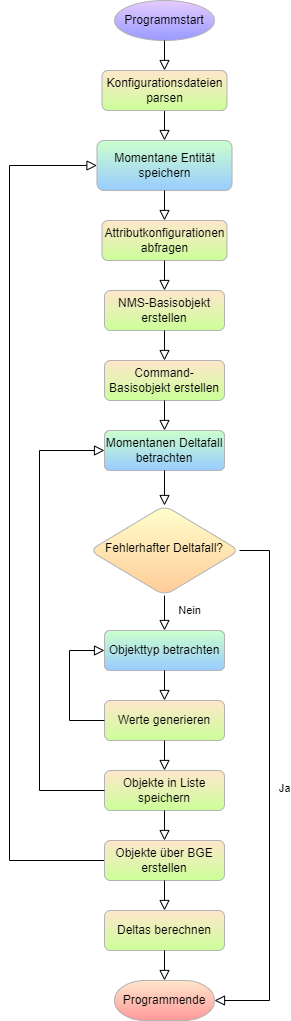
\includegraphics[height=.9\textheight]{tdg_konzept_flowchart.drawio.png}
    \caption{Konzeptioneller Programmablaufplan für die Datengenerierung\footnotemark}
\end{figure}

\newpage
\begin{enumerate}
    \item \textbf{Parsen der Dateien.} Der erste Schritt in einem Programmablauf, welcher eine von Konfigurationsdateien abhängige Ausführung beinhaltet, ist das Parsen ebendieser Dateien. Hierfür bietet Java verschiedene Möglichkeiten, welche im Kapitel \ref{ch:realisierung} weiter erläutert werden. Die Konfigurationen werden daraufhin in Java-Datenstrukturen, es bieten sich hierbei Listen oder Maps an, gespeichert, sodass über den restlichen Verlauf der Datengenerierung einfach auf die dort hinterlegten Werte zugegriffen werden kann.
    \item \textbf{Äußere Schleife: Iterieren über die Entitäten.} Die einzelnen Entitäten sollen getrennt voneinander betrachtet werden. Dies hat den Grund, dass so Basisattribute und \ac{BGE}-\ac{REST}-Pfade innerhalb eines Schleifendurchgangs nur einmal definiert werden müssen und für alle benötigten Testdaten einer Entität wiederverwendet werden können. Außerdem bietet diese Herangehensweise eine gute Übersichtlichkeit und erleichtert auch wesentlich das Debugging des Programms, da leicht abgeschätzt werden kann, an welchem Punkt die Programmausführung steht und wo es zu Fehlern kommt. Für jede Entität wird zu Beginn der Entitätsname in einer Variablen gespeichert, sodass auf diesen leicht zugegriffen werden kann. Der Name muss dabei eventuell erst korrekt formatiert werden, um ihn auch zur Tätigung von \ac{BGE}-Aufrufe nutzen zu können.
    \item \textbf{Abfragen der Entitätsattribute.} Das Abfragen der Attribute für eine Entität stellt einen Kernpunkt der Datengenerierung dar, da jede Entität individuelle Attribute hat, die sie definieren und die von \textit{Command} erkannt werden müssen. Es muss also genau bekannt sein, welche Attribute eine Entität benötigt, um ein valides Objekt davon in \textit{Command} erstellen zu können. Hierzu kommt die Schwierigkeit, dass sich Objekte der gleichen Entität in \ac{NMS}-Tabellen und \textit{Command}-Tabellen in ihren Attributen unterscheiden. Ein Beispiel hierfür ist das Typen-Attribut der Entität Chassis. Heißt es in einer \ac{NMS}-Umgebung einfach \enquote{commandType} und wird mit einem einfachen String, dem Namen des Chassistyps in \textit{Command}, befüllt, so nennt sich das korrespondierende Attribut für ein Objekt, welches in \textit{Command} zu erstellen ist, \enquote{createLinkDeviceMaster} und erfordert ein weiteres Unterattribut namens \enquote{linkedElid}, welches dann mit dem \ac{Elid}-String des Typen befüllt wird.
    
    Es ist möglich, die Attribute von \ac{NMS}-Entitäten über die \ac{BGE} abzufragen; hierfür existiert der folgende \ac{REST}-Endpunkt: 
    \begin{center}
        \textit{/rest/entity/cifEntityConfiguration/\{entityElid\}/QueryCifAttributeConfiguration}
    \end{center}
    
    Als Pfadparameter wird die \ac{Elid} der gewünschten Entität übergeben. Diese kann über einen weiteren Endpunkt \textit{cifEntityConfiguration/query} erhalten werden, indem im \ac{JSON}-Body der Anfrage der Entitätsname als Beschränkung angegeben wird. Die Antwort auf die Anfrage der Attribute liefert für jedes definierte Attribut eine Attributkonfiguration in \ac{JSON}-Form zurück, die das Attribut näher beschreibt. So wird beispielsweise für jedes Attribut angegeben, ob es für die Deltaberechnung verwendet wird, ob es ein Pflichtattribut ist und auch der korrespondierende Name des Attributs in der \textit{Command}-Umgebung wird bei einigen Attributen dort dokumentiert. Dies kann später zur Akkumulation der \textit{Command}-relevanten Attribute verwendet werden. Im Folgenden ist beispielhaft eine Attributkonfiguration für das Attribut \enquote{nmsId} angegeben.

    \begin{lstlisting}[caption=Attributkonfiguration für das Chassis-Attribut \enquote{nmsId}, label=nmsId-Konfiguration,language=json]
        {
            "commandAttribName": "VISIBLE_ID",
            "msgId": 50009,
            "attrName": "NMS_ID",
            "locked": "Y",
            "synchronizeToCommand": "Y",
            "catalogName": "CIF",
            "deltaCalculation": "N",
            "required": "Y",
            "dataLength": 200,
            "dataType": "VARCHAR",
            "remark": null
        }
    \end{lstlisting}

    \item \textbf{Erstellen von Basisobjekten.} Um valide Testobjekte einer Entität zu erstellen, muss die Datengenerierung sich an bestätigt validen Referenzobjekten orientieren. Eine sehr einfache Möglichkeit, dies zu erreichen, ist das dauerhafte Platzieren jeweils eines Dummy-Objekts in der \ac{NMS}- und \textit{Command}-Tabelle. Die Existenz dieser Objekte in den Tabellen allein dient als Validierung der Attribute und für tatsächliche Testobjekt müssten nur noch Werte abgeändert werden. Jedoch widerspricht diese Vorgehensweise den in Kapitel \ref{sec:anforderungen} formulierten Anforderungen, wonach alle durch die Testausführung erstellten Objekte in \textit{Command} oder den \ac{NMS}-Tabellen nur für die Zeit des Testlaufs bestehen und danach wieder bereinigt werden sollen. Weiterhin müssten für jede neue Testinstanz und darauf für jede Entität zwei Dummy-Objekte manuell und statisch erstellt werden, was dem grundsätzlichen Prinzip der Testdatengenerierung entspricht, sich von den statisch niedergeschriebenen Testdaten loszusagen.
    
    Stattdessen sollen die Basis- oder Referenzobjekte in jedem Testlauf dynamisch neu konstruiert und nicht dauerhaft in \textit{Command} erstellt werden. Für \ac{NMS}-Objekte ist dies über die im vorherigen Schritt abgefragten Attributkonfigurationen möglich. Es werden bis auf wenige Ausnahmen nur die Attribute benötigt, die in ihrer Konfiguration mit \colorbox{background}{\lstinline{\"synchronizeToCommand\": \"Y\"}} als relevant für die Vorgänge im \ac{CIF} gekennzeichnet sind. Durch das Abfragen der Attribute wird gewährleistet, dass das Basisobjekt aus tatsächlich existierenden Attributen zusammengesetzt wird und keine Fehler durch veraltete statische Daten oder gar Schreibfehler auftauchen können. Auch für \textit{Command}-Objekte soll ein Basisobjekt geschaffen werden. Dieses kann sich, wie schon im Punkt 3. erwähnt, teilweise auch aus den Attributkonfigurationen der \ac{NMS}-Attribute über den Wert im Feld \textit{commandAttribName} zusammensetzen. Dies trifft aber nicht auf jedes benötigte Attribut zu. Die restlichen Command-Attribute müssen also auf anderem Wege abgefragt werden. Eine Möglichkeit hierfür ist der wiederholte Versuch des Erstellens des Basisobjekts in \textit{Command}. Fehlt noch ein Attribut, wird dies eine Fehlermeldung zurückliefern, welche Rückschlüsse auf das noch fehlende Attribut enthält. So können Stück für Stück die fehlenden Attribute dem Objekt hinzugefügt werden. Kann es erfolgreich in \textit{Command} erstellt werden, ist das Objekt valide und kann als Basisobjekt verwendet und sogleich wieder aus \textit{Command} gelöscht werden.
    \item \textbf{Mittlere Schleife: Iterieren über die Deltafälle.} In diesem Schritt werden für die Entität die Deltafälle einzeln betrachtet. Dies erlaubt, ähnlich wie beim einzelnen Betrachten der Entitäten, das Wiederverwenden von bestimmten Daten, was für die korrekte Erkennung von Deltafällen in \textit{Command} notwendig ist. Das ganze Prinzip der Deltaberechnug beruht darauf, dass die Einträge in den verschiedenen Tabellen über gleiche Attributwerte als zusammengehörig erkannt werden. Das betrifft insbesondere das Attribut \textit{nmsId} beziehungsweise das \textit{Command}-Äquivalent \textit{visibleId}.
    
    An dieser Stelle kann auch eine Validierung der in der Entitäts-Konfigurationsdatei angegebenen Deltafälle durchgeführt werden. Falsch formulierte oder nicht existierende Deltafälle sollen abgefangen werden, da für diese keine Datengenerierung ausgeführt werden kann.
    \item \textbf{Innere Schleife: Iterieren über die Testobjekttypen.} Für jeden Deltafall gibt es verschiedene Typen von Objekten, die generiert werden müssen und in der Deltafall-Konfigurationsdatei spezifiziert sind. Die verschiedenen Typen beziehen sich dabei auf die verschiedenen Tabellen beziehungsweise den Status eines Objekts in \textit{Command}. Mögliche Objekttypen sind:
    \begin{itemize}
        \item nms
        \item command
        \item planningCreate
        \item planningDelete
    \end{itemize}

    Objekte mit Typ \enquote{nms} werden vom \ac{NMS}-Basisobjekt ausgehend generiert und später in die der Entität zugeordneten \ac{NMS}-Tabelle platziert. Basierend auf dem \textit{Command}-Basisobjekt werden Objekte mit Typ \enquote{command} direkt in \textit{Command} erstellt und besitzen dadurch den Planungsstatus \enquote{ACTUAL}. Objekte vom Typ \enquote{planning-} sind im Prinzip \enquote{command}-Objekte, werden aber mit zuvor aktiviertem Planning Protocol erstellt (\enquote{planningCreate}) beziehungsweise gelöscht (\enquote{planningDelete}) und besitzen so jeweils den Planungsstatus \enquote{PLANNED\_CREATED} oder auch \enquote{PLANNED\_DELETED}. Das Aktivieren eines Planning Protocols versetzt den User in \textit{Command} in den Planungsmodus. Wenn in diesem Modus Objekte erstellt oder gelöscht werden, übernimmt \textit{Command} diese Änderungen nicht direkt, sondern platziert diese Objekte mit einer speziellen Markierung, dem Planungsstatus, in \textit{Command}. Erst bei der Synchronisation der Daten werden die tatsächlichen Aktionen - das Erstellen oder Löschen eines Objekts - dann ausgeführt.

    Beim Generieren dieser verschiedenen Objekte soll nur das erste Objekt pro Deltafall vom Basisobjekt aus komplett neu mit Werten befüllt werden. So können unnötige Schleifeniterationen über alle einzelnen Attribute der Folgeobjekte vermieden werden; das zuerst generierte Objekt wird selbst zum Referenzobjekt und nachfolgende Objekte müssen nur noch wenige Werte geringfügig abändern. Somit ist auch garantiert, dass alle Testobjekte für einen Deltafall dieselben Werte für das \textit{nmsId}- beziehungsweise das \textit{visibleId}-Attribut besitzen. Nach der vollständigen Generierung eines Objekts wird dieses in einer Liste gespeichert, welche alle generierten Objekte sammelt.
    \item \textbf{Generieren von Werten.} Die Wertegenerierung selbst ist neben dem Konstruieren eines validen Basisobjekts der wichtigste Teil der Testdatengenerierung. Es ist essentiell, dass die Testdaten mit Werten gefüllt werden, die möglichst real sind, um die Kunden-Use-Cases auch tatsächlich abzudecken. (REFERENZ AUF UMFRAGE) Mithilfe von Utils-Methoden für die verschiedenen möglichen Attributarten sollen realistische Werte für alle Attribute erzeugt werden. Beispielsweise kann eine Methode speziell zur Generierung von \textit{visibleId}-Werten existieren, welche eine aussagekräftige ID zurückliefert, die sich aus Entität und Deltafall zusammensetzt. Insgesamt sollen zunächst Methoden zur Generierung von folgenden Attributarten implementiert werden:
    \begin{itemize}
        \item IDs
        \item Source Systems
        \item IP-Adressen
        \item Hardwareversionen
        \item Softwareversionen
        \item Anmerkungen
        \item Seriennummern
        \item Gerätetypen
    \end{itemize}

    Die Problematik bei den verschiedenen Attributarten besteht darin, dass in der Attributkonfiguration keine Aufschlüsse darauf gegeben werden, welches genaue Format ein Attribut verlangt. Lediglich die Datentypen der Attribute können ausgelesen werden, wobei diese zumeist einfache Strings sind. Die Unterscheidung der Attribute und der benötigten Werte kann daher nur über den Attributnamen geschehen. Hiefür soll die Herangehensweise mit Utils-Methoden gewählt werden, da diese sehr anschaulich und möglichst simpel ist. Je nach Attributnamen kann einfach die entsprechende Methode aufgerufen werden.
    \item \textbf{Erstellen der Testobjekte über die \ac{BGE}.} Nach der Generierung existieren sämtliche Testobjekte lediglich als Java-Objekte. Sie müssen dementsprechend noch in die korrekten Tabellen gefüllt werden. Dies geschieht über \ac{REST}-Aufrufe der \ac{BGE}. \ac{NMS}-Objekte könen über den \ac{REST}-Endpunkt \textit{\{nmsentity\}/bulkCreate} direkt als Gruppe von Objekten gleicher Entität über einen einzigen Aufruf erstellt werden. Die restlichen Objekte müssen jedoch einzeln erstellt werden. Hierfür gibt es je nach Entität mehrere Möglichkeiten. Manche Objekte können über den Endpunkt \textit{\{entity\}/create} direkt erstellt werden, während andere, beispielsweise das Chassis, in einem Kabinett, einem Slot, einem Lagerhaus oder einer Zone platziert werden müssen. Im Fall des Chassis ist zunächst nur die Zone relevant, weshalb hier der Endpunkt \textit{\{entity\}/placeInZone} zu verwenden ist. Vor dem Erstellen oder Löschen von Testobjekten vom Typ \enquote{planningDelete} oder \enquote{planningCreate} muss das Planning Protocol aktiviert werden. Dies ist ebenfalls über die \ac{BGE} möglich; hierzu existiert der \ac{REST}-Endpunkt \textit{planningProtocol/\{protocolElid\}/activate}. Für den Objekttyp \enquote{planningCreate} werden die Objekte dann wie normale \textit{Command}-Objekte erstellt, während Objekte vom Typ \enquote{planningDelete} über den Endpunkt \textit{\{entity\}/\{elid\}/delete} gelöscht werden müssen. Abschließend wird das Planning Protocol wieder deaktiviert
    \item \textbf{Berechnen der Deltas.} Der letzte Schritt in der erfolgreichen Generierung von Testdaten ist die Berechnung der Deltas, also der Diskrepanzen zwischen \ac{NMS}- und \textit{Command}-Tabellen. Hierfür wird ein eigens für die automatisierten Tests erstellter Testjob ausgeführt, der sämtliche Deltas im Source System der automatisierten Tests berechnet. Auch dieser Aufruf geschieht direkt aus dem Code über die \ac{BGE} mit dem \ac{REST}-Endpunkt \textit{\{jobName\}/startJobSync}. 
\end{enumerate}


